\begin{figure}[H]
    \centering
    \begin{subfigure}{0.24\textwidth}
        \centering
        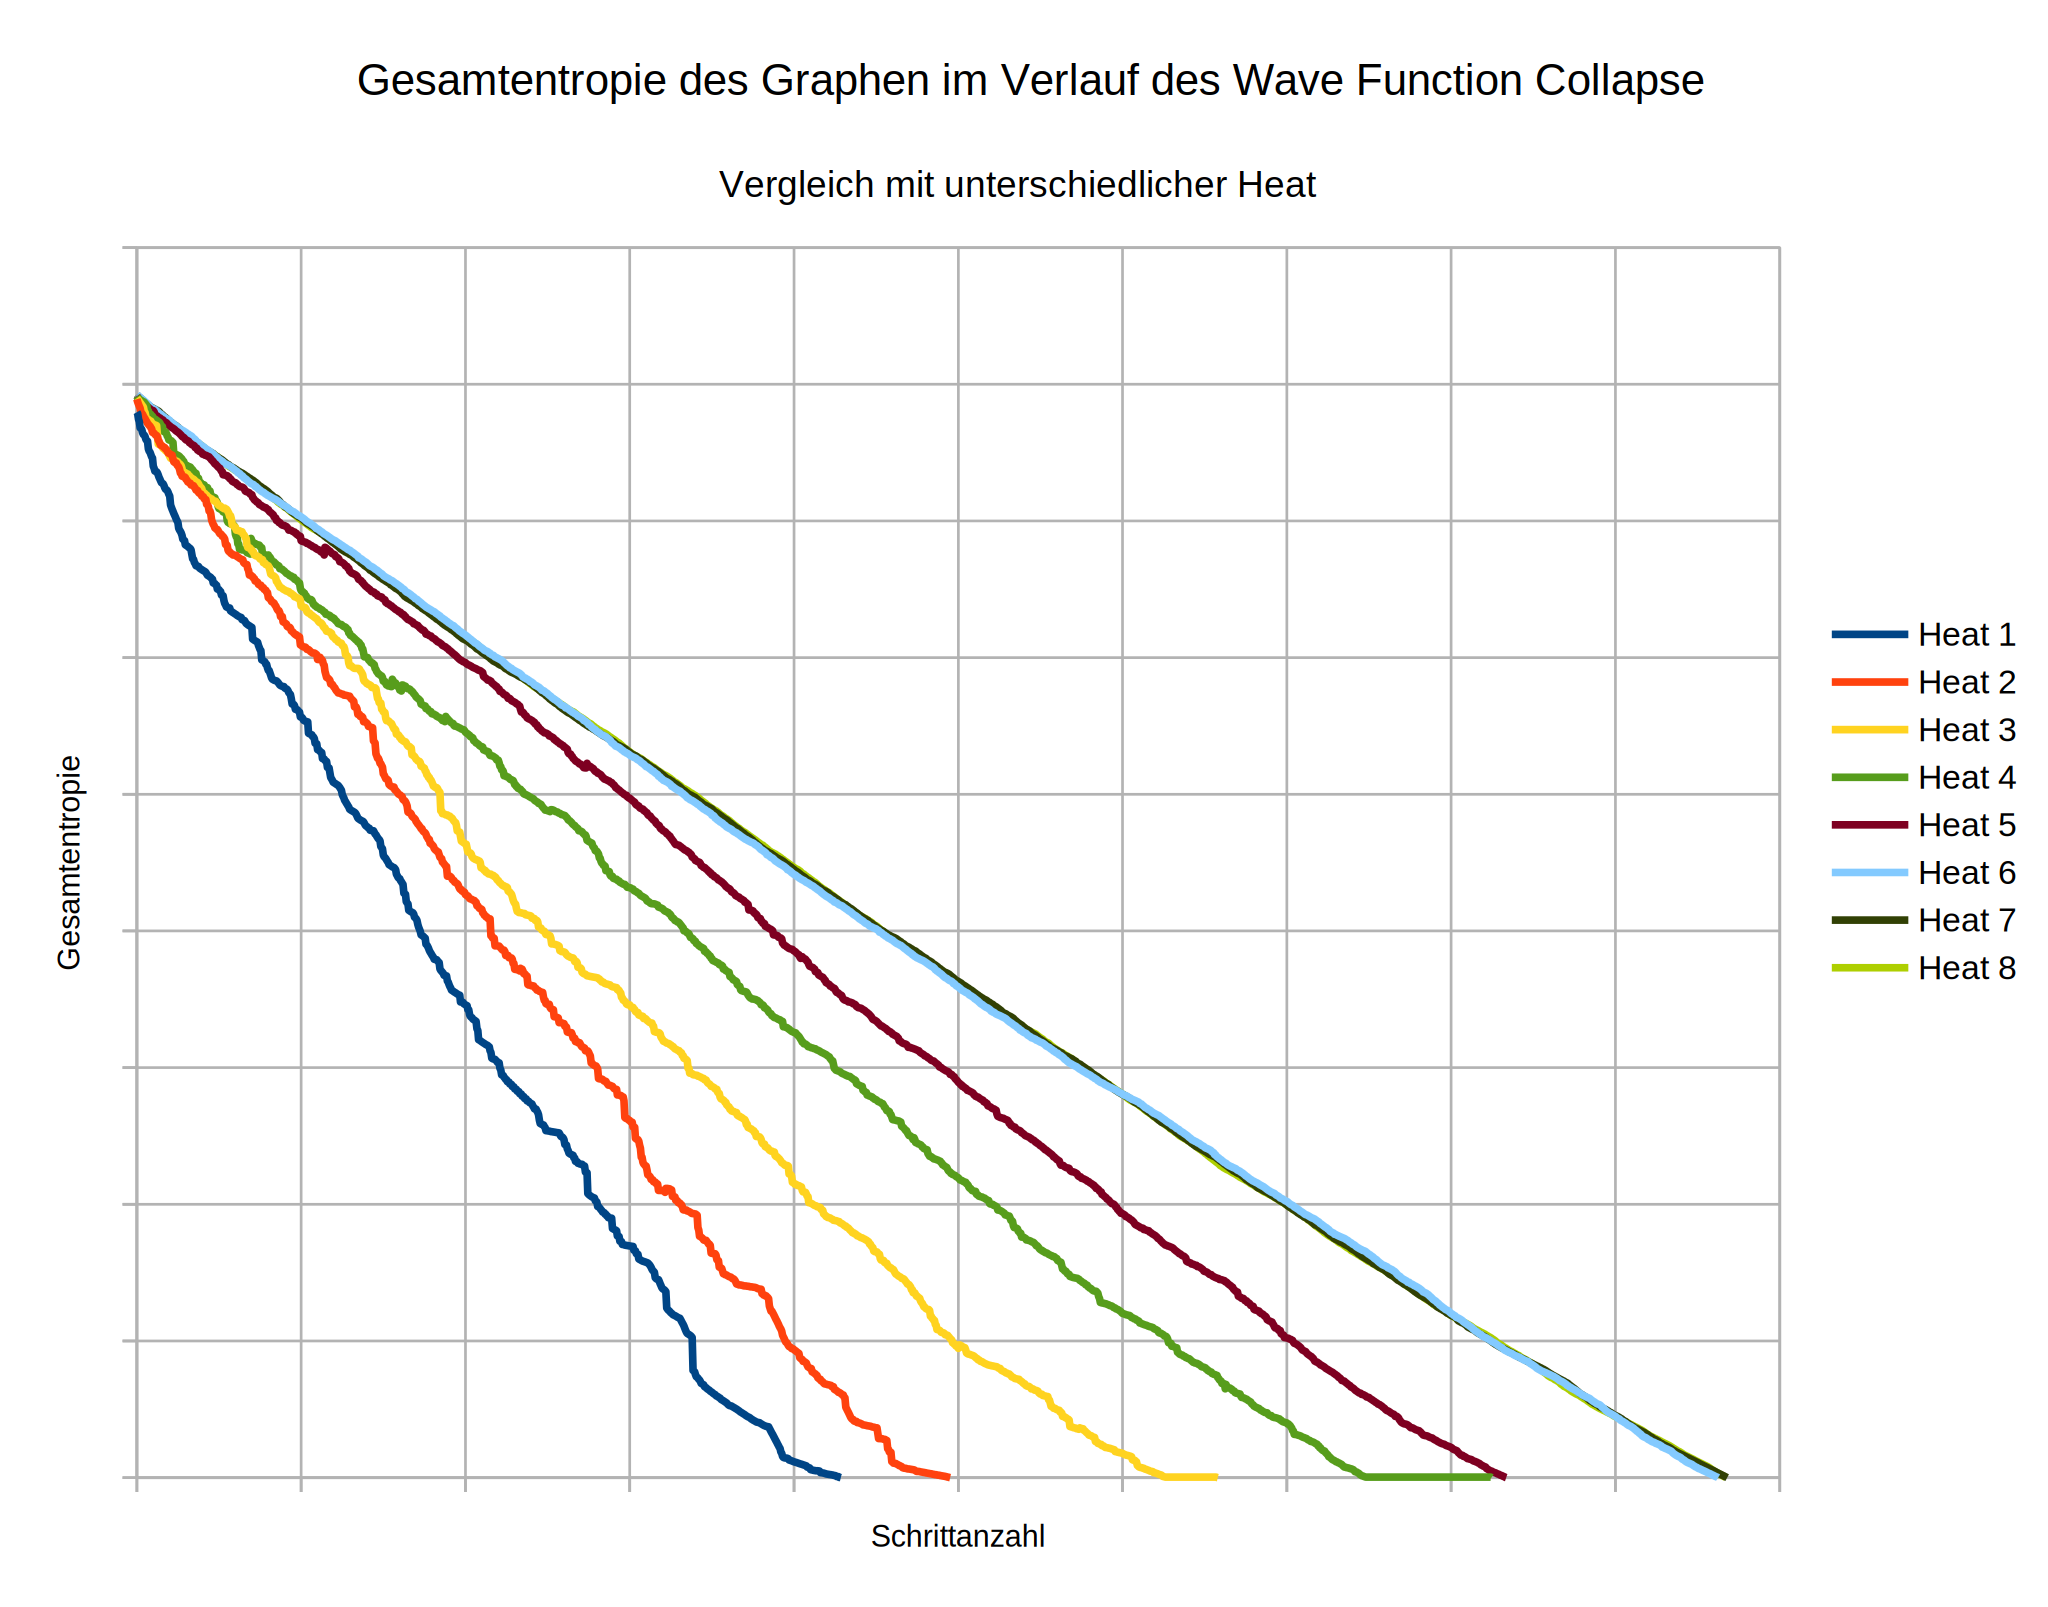
\includegraphics[width=\linewidth]{data/extract_wrapping/1.png}
        \caption{Umfeld 1}
    \end{subfigure}\hfill
    \begin{subfigure}{0.24\textwidth}
        \centering
        \includegraphics[width=\linewidth]{data/extract_wrapping/2.png}
        \caption{Umfeld 2}
    \end{subfigure}
    \begin{subfigure}{0.24\textwidth}
        \centering
        \includegraphics[width=\linewidth]{data/extract_wrapping/3.png}
        \caption{Umfeld 3}
    \end{subfigure}\hfill
    \begin{subfigure}{0.24\textwidth}
        \centering
        \includegraphics[width=\linewidth]{data/extract_wrapping/4.png}
        \caption{Umfeld 4}
    \end{subfigure}\hfill
    
    \vspace{4mm}
    
    \begin{subfigure}{0.32\textwidth}
        \centering
        \includegraphics[width=\linewidth]{data/extract_wrapping/5.png}
        \caption{Zustand 1}
    \end{subfigure}\hfill
    \begin{subfigure}{0.32\textwidth}
        \centering
        \includegraphics[width=\linewidth]{data/extract_wrapping/6.png}
        \caption{Zustand 2}
    \end{subfigure}
    \begin{subfigure}{0.32\textwidth}
        \centering
        \includegraphics[width=\linewidth]{data/extract_wrapping/7.png}
        \caption{Zustand 3}
    \end{subfigure}\hfill
    
    \caption{
        Extraktion mit N=3 und vertikalem Wrapping. 
        \\(d) Umfeld 4 überschreitet den Rand und nimmt die Pixel aus der ersten Reihe.
        \\(e) Umfeld 1 ergibt einen Zustand 1 mit einer Frequenz von 1.
        \\(f) Umfeld 2 und 3 sind gleich, somit wird nur ein Zustand mit einer Frequenz von 2 erstellt.
    }
    \label{fig:extract_wrapping}
\end{figure}